%!TEX program = xelatex
\documentclass[12pt]{article}
\usepackage{authblk}
\usepackage[margin=2cm]{geometry}
\usepackage[table,xcdraw]{xcolor}
\usepackage{booktabs}
\usepackage{bookmark}
\usepackage{graphicx}
\usepackage{float}
\usepackage{subfigure}
\usepackage{url}
\usepackage{amsmath}
% \usepackage[hidelinks]{hyperref}
\usepackage{xeCJK}
\usepackage{fontspec}
\usepackage{setspace}
\usepackage{fancyhdr}
\usepackage{titling}
\usepackage{caption}
\usepackage{enumerate}
\setmainfont{Minion Pro}
\setCJKmainfont{宋體-繁}
\renewcommand{\baselinestretch}{1.2}
\newcommand{\upcite}[1]{\textsuperscript{\textsuperscript{\cite{#1}}}}
% \setlength{\droptitle}{5cm}
% \pagenumbering{gobble}

\pagestyle{fancy}
\fancyhf{}
\fancyhead[LE,RO]{B09704016, 經濟三張茗傑}
\fancyhead[RE,LO]{Econometric (I) HW6}
\rfoot{\thepage}

\setlength{\headheight}{13pt}
\geometry{a4paper,left=1.75cm,right=1.75cm,top=2.75cm,bottom=2cm}
\begin{document}

\section*{Question 1}
\begin{enumerate}[(a)]
    \item 135 firms are used in the estimation.
    \item Receiving grants increased  29.120188 hours of training per employee. 
    The coefficient is significant since p-value $\approx$ 0.
    \item we modify our model by replacing $grant_{it}$ with $grant\_first_{it}$ and $grant\_second_{it}$, namely
    $$hrsemp_{it} = \beta_0 + \beta_1 \cdot grant\_first_{it} + \beta_2 \cdot grant\_second_{it} + \alpha_i + \delta_1 \cdot year_{1t} + \delta_2 \cdot year_{2t} + e_{it}$$
    where $grant\_first_{it}$ indicates whether the firm was in the first year of grants (no matter the firms received grants in 1988 or 1989), while $grant\_second_{it}$ indicates whether the firm was in the second year of grants (the firms must receive grants in 1988).
    \item The coefficient of $grant\_first_{it}$ is statistically significant 34.228179, while the coefficient of \\ 
    $grant\_second_{it}$ is statistically insignificant 0.50408042. This result means that the effect of grants were generally restricted to the year they were distributed, 
    implying the long-term effect of this policy was small.
\end{enumerate}

\section*{Question 2}
\begin{enumerate}[(a)]
    \item The dependent variable is $win\_dem\_t1$. \\ 
    The running variable is $demvoteshare$. \\ 
    The treatment is $win\_dem$. \\ 
    This is a sharp RDD with the cut-off threshold of $demvoteshare = 0.5$. \\ 
    \begin{figure}[H]
        \centering
        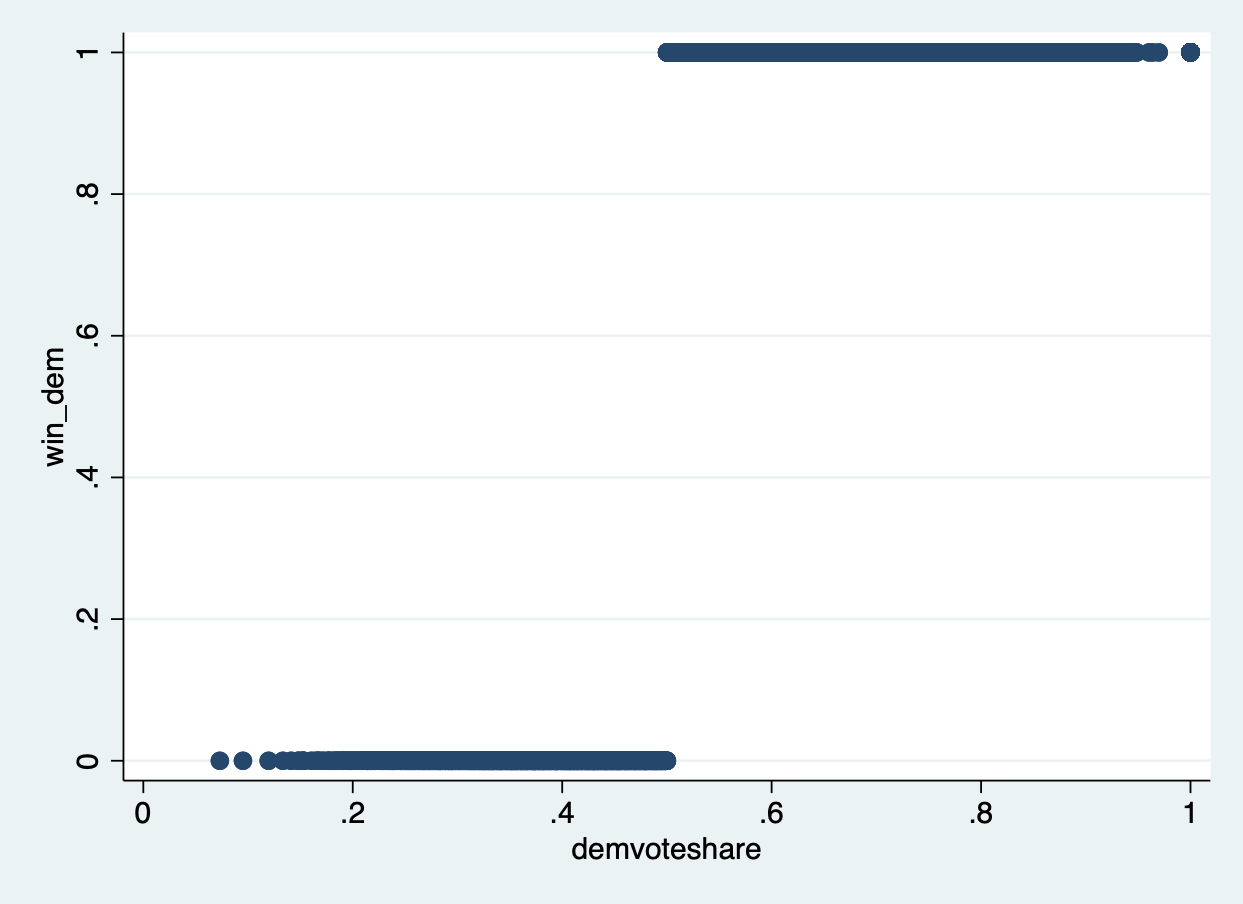
\includegraphics[width=0.65\textwidth]{RDD scatter.jpg}
    \end{figure}
    \item Observations with $win\_dem = 1$ are largely different from observations with $win\_dem = 0$, that is, treatment and control groups are not "randomized". 
    The estimation will be biased since regions with $win\_dem = 1$ are composed of more voters preferring Democrats.
    \item The jump is estimated to be {\color{red}?}
    \begin{figure}[H]
        \centering
        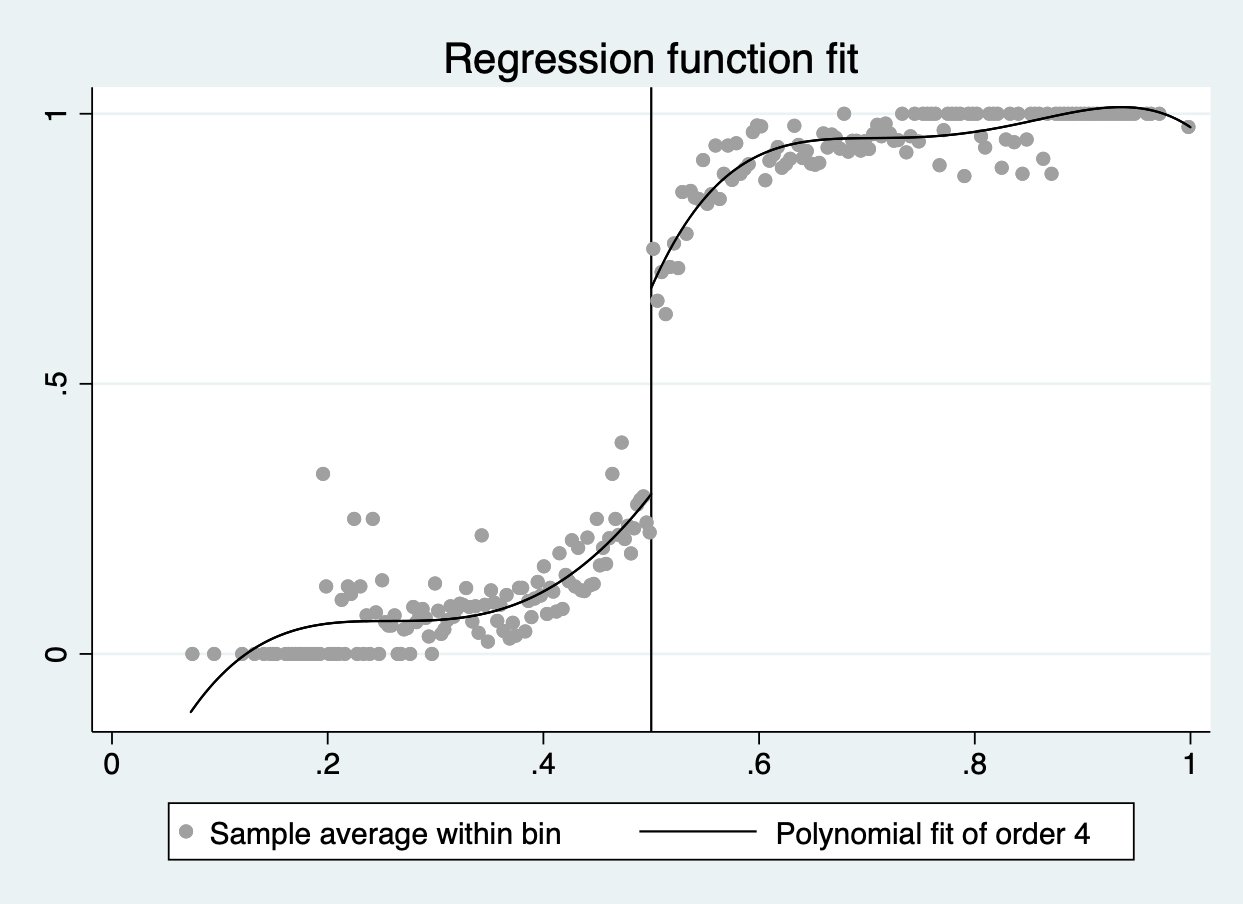
\includegraphics[width=0.65\textwidth]{RD plot.jpg}
    \end{figure}
\end{enumerate}

\end{document}